\section{Results}
\label{sec:results}
\subsection{Structural Profiles: Motif and Size}
\begin{figure*}[t]
\centering
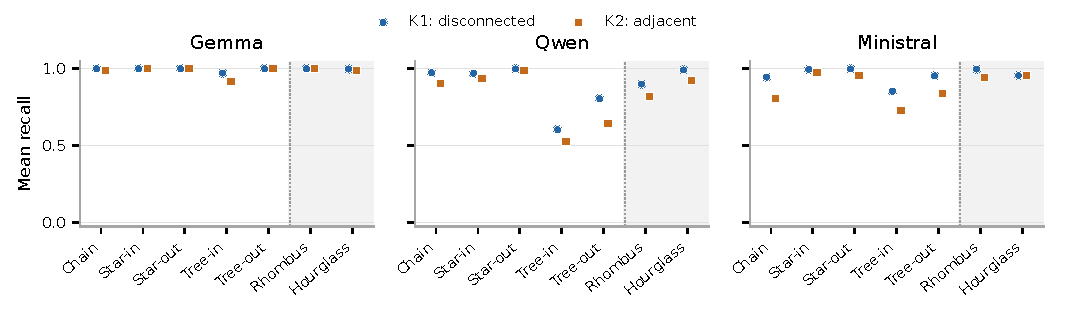
\includegraphics[width=\textwidth]{figures/recall_motifs.pdf}
\caption{Core recall with explicit source-card relations: K1 disconnected and K2 adjacent distractors, 100 planned tasks per point. The first five families have six nodes; shaded rhombus/hourglass use four/five and are not equal-size contrasts. Invalid outcomes contribute zero. These are descriptive macro means, without inferential error bars.}
\Description{Recall across seven graph-pattern families for three models. Incoming-tree recall is below outward-star recall, with model-dependent changes under adjacent contexts.}
\label{fig:motifs}
\end{figure*}
Figure~\ref{fig:motifs} shows task-family differences at a common reference size. Under K1, six-node incoming-tree recall is 0.972 for Gemma, 0.603 for Qwen, and 0.853 for Ministral. Outward stars are close to complete coverage. The common size does not eliminate differences in query semantics, relation types, or sampled entities; it rules out a node-count-only description of these observed task profiles, not every competing explanation.

Precision supplies a different view. Qwen's K1 incoming-tree precision is 0.988, despite recall of 0.603 and exact recovery of 0.150. It often selects a small, mostly reference-consistent set while failing to cover the reference. Gemma's corresponding precision is 1.000 and exact 0.870. Appendix~\ref{app:conditions} reports precision profiles separately rather than combining the two quantities into one F1 curve.

\begin{figure*}[t]
\centering
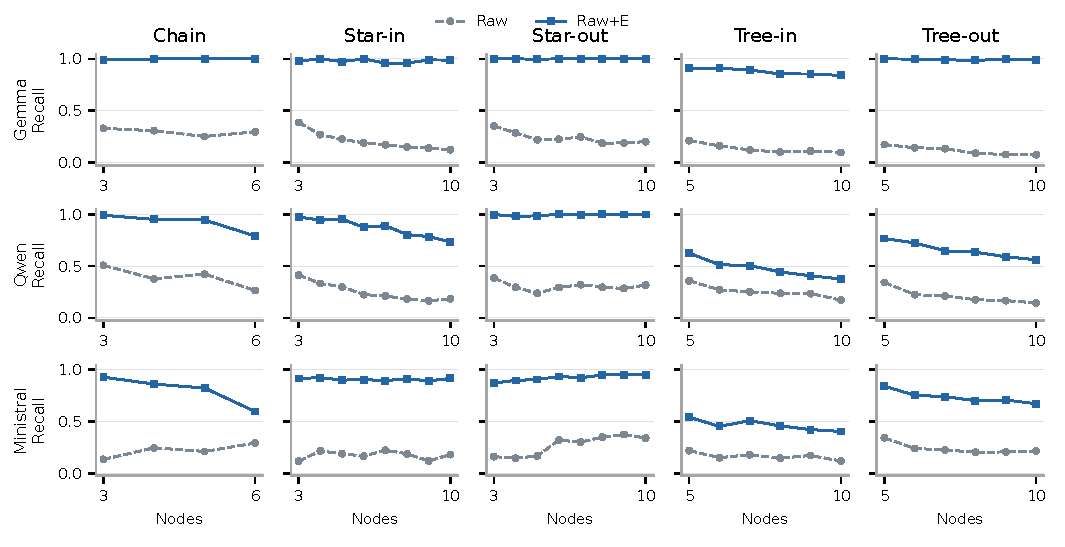
\includegraphics[width=\textwidth]{figures/recall_sizes.pdf}
\caption{Recall across all variable-size families and all three models in Full Raw/Raw+E. Each point has 100 planned tasks and 25 candidates, with invalid outcomes contributing zero. Raw+E adds relations. Sizes are different frozen cohorts, not paired expansions; target prevalence and distractor count change with size. No universal monotonicity or isolated size effect is claimed.}
\Description{Fifteen panels compare Raw and Raw+E recall against subgraph size. Incoming trees and some chains decline, while outward stars often remain near complete coverage.}
\label{fig:sizes}
\end{figure*}
Size sensitivity also depends on family and model (Figure~\ref{fig:sizes}). Under Raw+E, chain recall changes from 0.990 at three nodes to 0.790 at six for Qwen, and from 0.927 to 0.595 for Ministral. Gemma changes from 0.990 to 1.000. Outward stars provide contrary profiles: Qwen changes from 0.997 at three nodes to 0.998 at ten, Gemma remains at 1.000, and Ministral changes from 0.870 to 0.950. These comparisons describe different accepted cohorts, not beneficial or harmful effects of adding a node to the same task.

Incoming-tree Raw+E recall is lower at ten than five nodes for all three models: 0.910 to 0.841, 0.624 to 0.375, and 0.540 to 0.403 for Gemma, Qwen, and Ministral. Intermediate values need not be monotonic. The fixed candidate pool also changes the proportion of reference entities as size increases. We therefore report the full profiles, including exceptions, rather than treating node count as an intrinsic complexity coefficient.

\subsection{Relation Availability and Matched-Fact Presentation}
\begin{table*}[t]
\caption{Descriptive paired changes in mean recall. Columns: Raw+E minus Raw (3,400 pairs/model); adjacent minus disconnected triples/text; text minus triples for procedural/direct queries; destination minus source; both cards minus source; direct minus procedural query (700 pairs/model for these Core contrasts). All planned outcomes are retained. No recall confidence intervals or significance tests were computed.}
\label{tab:effects}
\centering\small
\begin{tabular}{lrrrrrrrr}
\toprule
Model & \shortstack{Raw+E} & \shortstack{Adj.\\triples} & \shortstack{Adj.\\text} & \shortstack{Text\\steps} & \shortstack{Text\\direct} & \shortstack{Dest.} & \shortstack{Both} & \shortstack{Direct\\query} \\
\midrule
Gemma & +0.774 & -0.011 & -0.015 & -0.002 & -0.006 & +0.000 & -0.003 & +0.001 \\
Qwen & +0.519 & -0.071 & -0.064 & -0.035 & -0.035 & +0.005 & +0.059 & -0.003 \\
Ministral & +0.567 & -0.072 & -0.045 & -0.001 & -0.002 & -0.043 & -0.006 & -0.016 \\
\bottomrule
\end{tabular}

\end{table*}
Explicit relation disclosure substantially increases recall (Table~\ref{tab:effects}). Raw/Raw+E mean recall changes from 0.198 to 0.972 for Gemma, 0.278 to 0.798 for Qwen, and 0.218 to 0.785 for Ministral. The gains are 0.774, 0.519, and 0.567. Precision changes from 0.859 to 0.988, 0.885 to 0.975, and 0.459 to 0.976, respectively. High Raw precision can therefore coexist with low route coverage. Since native metadata is not verified sufficient for every route, low Raw recall is not automatically a failure to reason from available facts.

Matched-fact representation gives a more restricted diagnostic. Text-minus-triples recall differences for Qwen are $-0.035$ under both procedural and direct queries after rounding. Gemma and Ministral have smaller descriptive differences in those comparisons. Hosting effects are model-specific: duplicating facts yields a Qwen aggregate recall gain of 0.059, whereas Gemma and Ministral do not show the same positive direction. These are point estimates, not equivalence findings or newly tested interactions.

\begin{table}[t]
\caption{Mean recall on six-node Tree-in tasks: one model per row, conditions in columns. K1/K3/K4 host triples on source/destination/both cards with a procedural query; K7 uses source cards and a direct query. Each cell retains 100 planned tasks. Ministral has 99 valid outcomes in K3 and 91 in K7; every other cell has 100. Invalid outcomes contribute zero.}
\label{tab:treein}
\centering\small
\begin{tabular}{lrrrr}
\toprule
Model & K1 & K3 & K4 & K7 \\
\midrule
Gemma & 0.972 & 0.983 & 0.982 & 0.982 \\
Qwen & 0.603 & 0.603 & 0.802 & 0.660 \\
Ministral & 0.853 & 0.787 & 0.908 & 0.837 \\
\bottomrule
\end{tabular}

\end{table}
The focused incoming-tree comparison illustrates why aggregate changes need localization (Table~\ref{tab:treein}). Qwen's recall is 0.603 with source or destination hosting, 0.802 with both-card hosting, and 0.660 with a direct query. Ministral reaches 0.908 with both-card hosting, but destination hosting yields 0.787 versus 0.853 at source. Gemma remains near complete coverage in all four conditions. Thus moving incoming relations to destination cards does not universally improve selection, and a presentation change can affect models differently despite matched unique facts.

Saved Qwen selections provide an additional output-level check: 71 of 100 K1 incoming-tree outputs equal the anchor plus its first incoming neighbourhood. Under K4, 38 of those 71 become exact, while six of the 15 initially exact outputs lose exactness. Under K7, the one-hop count falls to 52, but total exact recovery changes only from 15 to 16. A reduction in one error signature can therefore include substitution into other errors. This is a post-hoc diagnostic of final sets, not a record of internal stopping; Gemma lacks the selected identities needed for this particular check.

\subsection{Adjacent Contexts}
Adjacent-minus-disconnected recall differences are negative for all three models in both triples and text contrasts (Table~\ref{tab:effects}). The motif profiles show where coverage remains incomplete under these conditions (Figure~\ref{fig:motifs}). Distractor identities and graph density also change in the paired noise variants. We therefore interpret these as archived context contrasts, not isolated causal effects of adjacency or evidence of a universal motif-by-noise interaction.
